%\documentclass[review]{elsarticle}
\documentclass[5p]{elsarticle}


\usepackage{lineno,hyperref}
\usepackage[separate-uncertainty=true,multi-part-units=single]{siunitx}
\usepackage{color}
\modulolinenumbers[5]
\usepackage{mhchem}
\usepackage{enumitem}

\journal{Geomorphology}


\newcommand{\COMON}{\begin{color}{blue}}
\newcommand{\COMOFF}{\end{color}}

%% APA style
\bibliographystyle{model5-names}\biboptions{authoryear}

\begin{document}


	\begin{frontmatter}

\title{Insights into the Paleo-elevation of Yosemite Valley Shortly after the Last Glacial Maximum.\\ \vspace{1cm}Insights into the Paleo-elevation of Yosemite Valley 15,000 years B.P. from the Royal Arches Meadow Rock Avalanche.\\ \vspace{1cm}Suggestions?}

%% Group authors per affiliation:
\author[Marcus]{Marcus Pacheco\corref{cor1}}
\address[Marcus]{California State University, Fresno}
\cortext[cor1]{Corresponding author.}
\ead{mvpacheco90@mail.fresnostate.edu}

\author[Alain]{Alain Plattner}
\address[Alain]{University of Alabama}

\author[Chris]{[Christopher Pluhar}
\address[Chris]{California State University, Fresno}

\author[Greg]{Greg Stock}
\address[Greg]{Yosemite National Park}



										\begin{abstract}
										
\COMON This is tjust a Test abstract!\COMOFF Since the retreat of the Last Glacial Maximum (~15,000 years ago), rockfalls have been the major force shaping Yosemite Valley, California. Rock avalanches are an especially large rockfall/rock slide that extends far beyond the cliff where they originate. These events are infrequent, but can reach hundreds of meters into the valley, and deposit an extremely large volume of debris when compared with regular rockfall events. Yosemite Valley is home of at least ten rock avalanche deposits, with the Royal Arches Meadow rock avalanche (RAMRA), situated in eastern Yosemite Valley, being the oldest event (~14,000 yr BP). Because this event occurred shortly after the Last Glacial Maximum (LGM), mapping the interface between this rock avalanche and the underlying valley sediments can give us insights about the valley elevation and overall geomorphic state of Yosemite Valley shortly after the LGM.  Holocene aggradation covers parts of the deposit, reducing its surface expression. This represents a challenge for estimating the dimensions of the deposit. To overcome this obstacle, we used a combination of geophysical methods (Electrical Resistivity Tomography (ERT) and Ground Penetrating Radar (GPR)) to image the interface between the RAMRA and underlying valley sediments. The strong dielectric permittivity and electrical resistivity contrast between the rock avalanche and the underlying sediments make both electrical resistivity tomography and ground penetrating radar ideal methods for our purpose. This then allowed us to infer that the surface of the valley underneath the Royal Arches Meadow Rock Avalanche is in average 1209m with a variation of +/- 3.2m.

									\end{abstract}

					\begin{keyword}
GPR \sep ERT \sep Yosemite
%\texttt{elsarticle.cls}\sep \LaTeX\sep Elsevier \sep template
%\MSC[2010] 00-01\sep  99-00
					\end{keyword}

	\end{frontmatter}

%\linenumbers

\section{Introduction}

Yosemite Valley, located in Yosemite National Park-CA, is famous for its kilometric near-vertical to overhanging walls. Most of those cliffs are constituted of resistant granitic rock (Bateman, 1992), and although they are composed of such resistant material, weathering and erosion throughout the geological time break them down, transporting this material towards the valley in form of rockfall, rock slides, debris flow, and rock avalanches. The record of such dynamic process became well preserved in Yosemite Valley since the retreat of the last glacier, locally known as Tioga. Due to the relatively low elevation of Yosemite Valley, it is likely that this portion of the park was free of ice by 15,000 years (Wieczorek and J\"ager, 1996). This then formed the glacial lake Yosemite, and it is possible that mass wasting deposits have been intercalating with fluvial, deltaic and lacustrine sediments from the glacial lake Yosemite stage.   In other words, the absence of moving glaciers, allied with the low gradient of the Yosemite Valley (~3m/km), created the perfect condition to preserve mass wasting deposits in the valley. 

Unlike Rockfall, which happen very frequently in the park and produce small volume of debris, rock avalanches are rare, and typically move large masses of material over long distances in a matter of seconds (Stock and Uhrhammer, 2010). Consequently, these events are an important geomorphic process reshaping the landscape of Yosemite Valley. 

While some of the rock avalanches and other mass wasting deposits in Yosemite Valley are well studied and mapped \COMON(e.g., Stock, Luco, et al., 2012;  Stock \& Uhrhammer, 2010; and Wieczorek, Morrissey, Iovine, \& Godt, 1998) \COMOFF, little is known about the Royal Arches Meadow Rock Avalanche (RAMRA). Cosmogenic \ce{^{10}Be} exposure ages demonstrate that the RAMRA happened \SI{14030 \pm 340}{yr\, B.P.} (G. Stock, personal communication). This makes this avalanche deposit the oldest dated rock avalanche in Yosemite Valley. More importantly, because the Royal Arches Meadow Rock Avalanche happened approximately at 14000 B.P., the interface between the bottom of the RAMRA and the underlying paleo-valley marks the elevation state of the valley shortly after the LGM \COMON(15,000 to 20,000 years ago)\COMOFF. 

Therefore, mapping this interface can give us insights about paleo-elevation of Yosemite Valley shortly after the LGM, and better understand of the local rates of aggradation. In addition, mapping the extent of the rock avalanche may provide valuable information for future research related to the dynamics of those events, because the runout extent of an avalanche, along with its associated volume and slope, are typically used to understand the event kinematics, which can also improve risk assessment (e.g., Wieczorek et al., 1999; Guzzetti et al., 2003; Stock, Luco, et al., 2012).





\section{Study Area}

Yosemite Valley, located in Yosemite National Park -- CA (Figure~\ref{Study_Area}A), is a ~1  km deep glacially carved canyon in the Sierra Nevada, California, USA (Matthes, 1930; Huber et al., 1987), home to some of the largest granitic rock faces in the world. Yosemite Valley is the home of at least ten rock avalanche deposits, and in this research,  we investigated the oldest of them, the Royal Arches Meadow rock avalanche (RAMRA) (Figure~\ref{Study_Area}B), situated in eastern Yosemite Valley. 

									\begin{figure*}[h]

	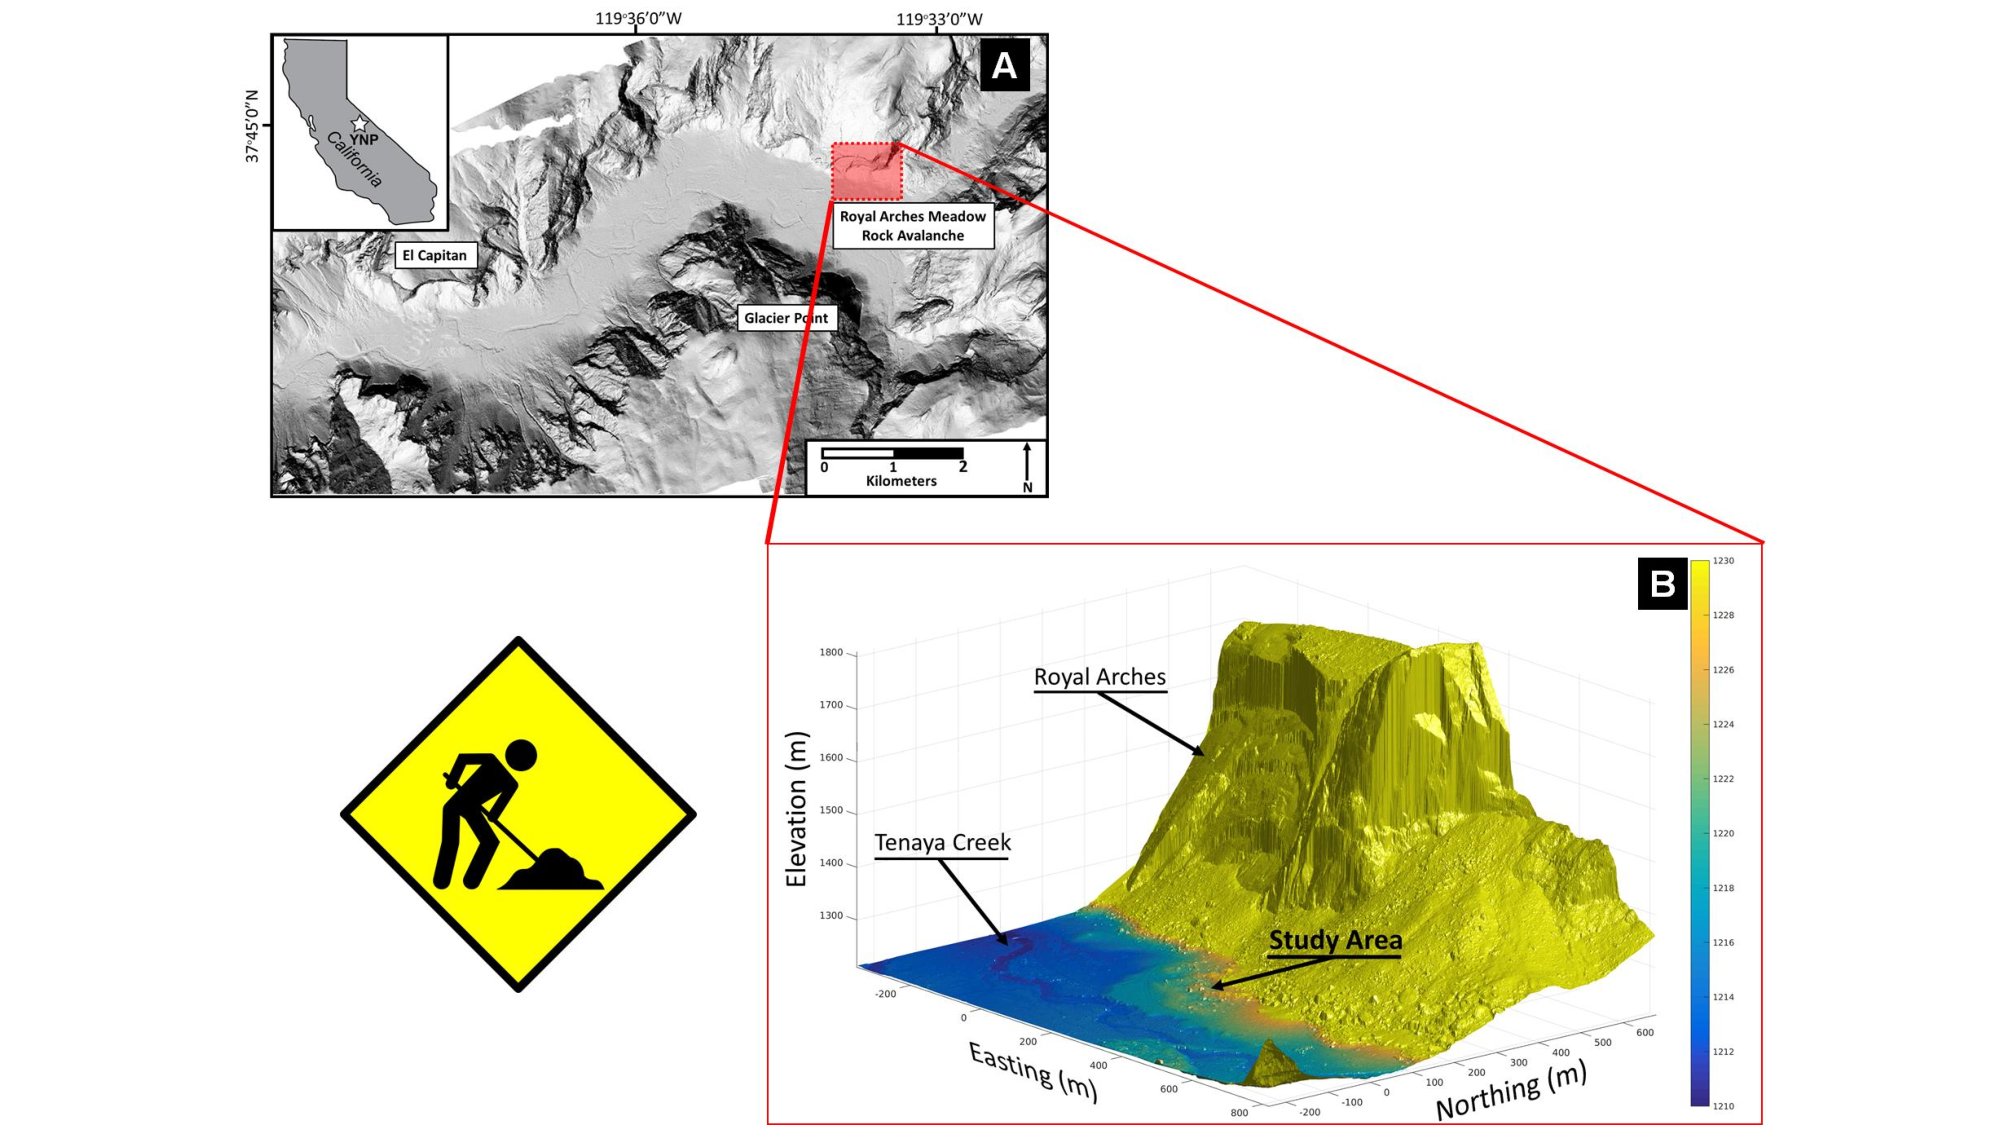
\includegraphics[width=\textwidth]{Figures/Study_Area.pdf}
		\caption{: (A) Map of view of Yosemite Valley - CA, red box highlights the study area (modified after Brody et al., (2015)). (B) oblique view of the study area. \label{Study_Area}}


									\end{figure*}

The proximal portion of the study area (NE), close to the talus deposits (yellow portion in (Figure~\ref{Study_Area}B) is marked by large boulders of several meters (Figure~\ref{Study_Area2} A and B). Moving towards the distal portion of the avalanche deposit (SW direction), we observed that the bolders decreaase in size and surficial expression (from several meters to centimeters scale) (Figure~\ref{Study_Area2} C and D), until they complete desapear in the southmost portion close to the Tenaya Creek cutbank (Figure 4 G).

\COMON
	Talk about topography here
	
	Possibky topographic profiles?
\COMOFF

									\begin{figure*}[h]

	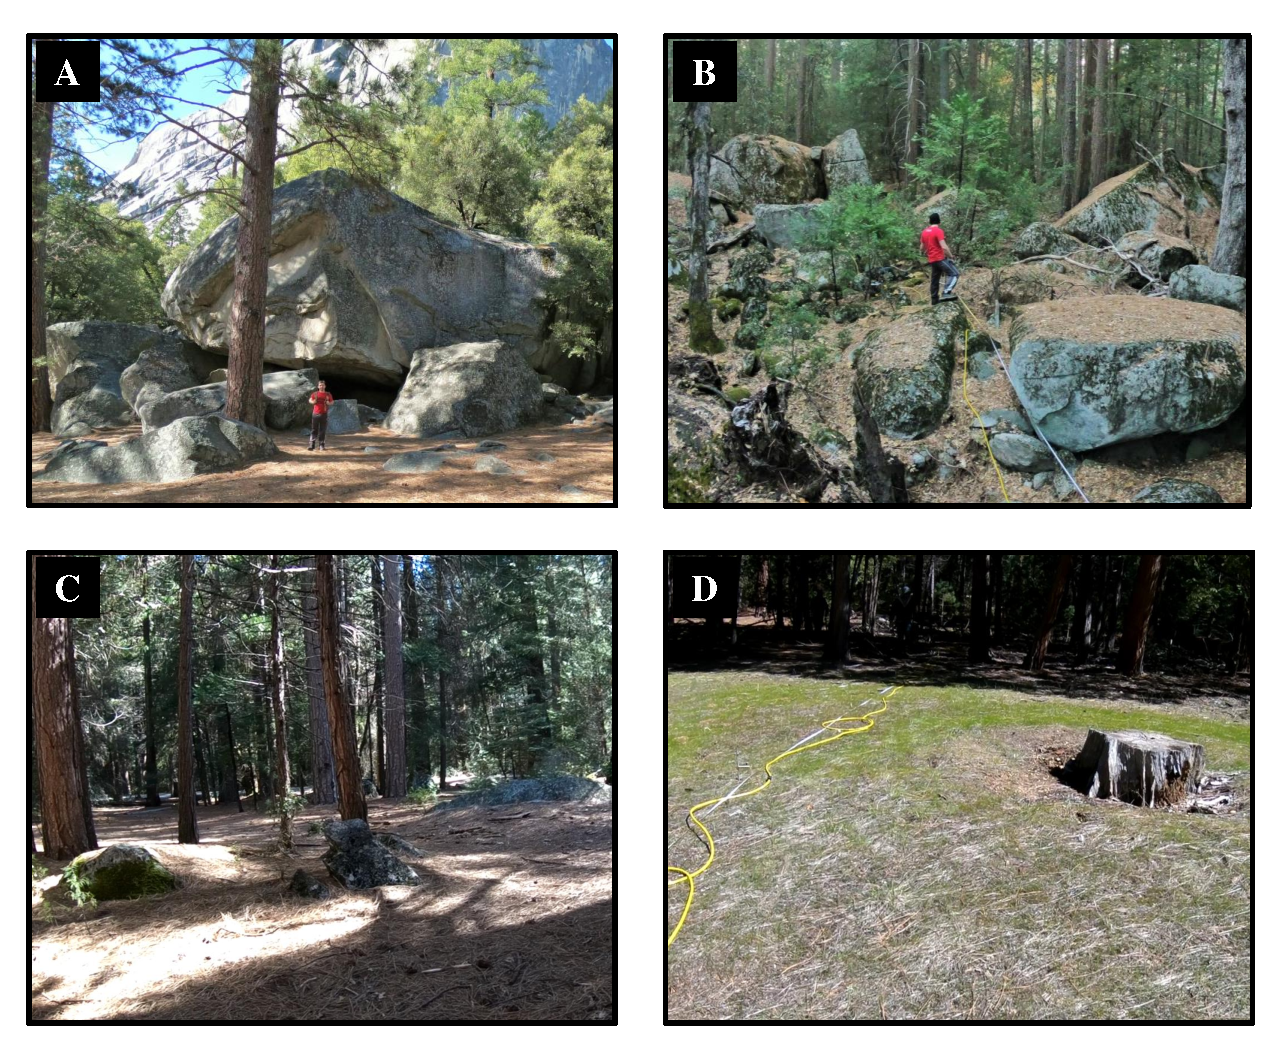
\includegraphics[width=\textwidth]{Figures/Study_Area2.pdf}
		\caption{: Surface morphology of the Royal Arches Meadow Rock Avalanche. Walking from the proximal portion (A-B) at NE, towards the distal portion (C-D) at SW. \label{Study_Area2}}

									\end{figure*}
			
A common strategy deployed to study, and map rock avalanche deposits is the combination of LiDAR and other topographic tools along with field observations. These techniques allow researchers to investigate surficial morphological expressions, as well as volume, and runout of rock avalanche deposits. As example, Wieczorek \& J\"ager (1996) estimated the volume of mass wasting deposits in Yosemite Valley using  a Digital Elevation Models (DEM) of the present topography, and  another DEM representing the hypothetical datum of the flat valley level soon after filling of glacial lake Yosemite. 

The second DEM is called hypothetical datum because the valley elevation that we walk today differs from the paleo-valley elevation existent after the LGM. In other words, to precisely estimate the volume of mass wasting deposit you would need to identify the top and the bottom of the deposit. The top of the deposit can be inferred from the current topography. However, the bottom of the deposit cannot be inferred as the modern valley floor, given that Yosemite Valley has been aggrading since the LGM. This idea can be supported when we analyze the surficial expression of deposits in the valley. The morphological surficial expressions of older deposits such as the Royal Arches Meadow rock Avalanche (\SI{\approx14}{\kilo a}) and the Glacier Point Rock Fall deposit (\SI{9.6 \pm 1}{\kilo a}) (Cordes et al., 2013) are faded when compared to more recent rock avalanches deposits such as the El Captain Rock Avalanche (\SI{\approx3.6}{\kilo a}) (Stock \& Uhrhammer, 2010). In addition, the work of Cordes et al., (2013) demonstrated that the Valley beneath the glacier point (Figure~\ref{Study_Area}) has aggraded approximately 5m since the LGM.

Therefore, to study the Royal Arches Meadow Rock Avalanche and to gain insights into the aggradation rates since the LGM we used a combination of geophysical methods to investigate the extent of the avalanche deposit and the interface between the bottom of the rock avalanche deposit and the paleo-valley elevation shortly after the LGM.



\section{Methods}

Geophysical methods have been successfully applied to image mass wasting deposits  (e.g., Sass, 2006; Otto \& Sass, 2006; Socco et al., 2010; Brody et al. 2015, Liu \& Plattner 2018), allowing researchers to better estimate volume, image internal structures, and to track lateral continuity in depth. In addition, Doetsch, Linde, Pessognelli, Green, \& G\"unther, (2012), have demonstrated the effectiveness of using Ground Penetrating Radar (GPR) to constrain electrical resistivity tomography (ERT). Inspired by these works, we combined ERT and GPR surveys to image the subsurface of the Royal Arches Meadow rock avalanche. These geophysical methods are highly suited to the area of study because of the strong dielectric permittivity and electrical resistivity contrast between the rock avalanche and the underlying valley floor. We georeferenced the geophysical data using differential GPS measurements acquired with a Trimble Geo 7X GPS, and the elevation information was extracted from LiDAR data.



	\subsection{Ground Penetrating Radar (GPR)}
										
Ground Penetrating Radar is a noninvasive geophysical technique that detects electrical discontinuities in the shallow subsurface (typically < 50 m) (Neal, 2004). The most common form of GPR measurements involves keeping a transmitter antenna and a receiver antenna at a fixed distance and moves them along a profile line on the surface to detect reflections from subsurface features (Jol, 2008). 

Eight GPR profiles were collected with a Sensors \& Software PulseEKKO Pro (50 and 100 MHz) system (Figure~\ref{GPR profile 7}). Profiles G1, G2, G3, G5, G6, G7 and G8 were collected with the 50 MHz antenna, while profile G4 was collected with the 100 MHz antenna. Note that due to obstacles in the field (e.g., boulders and fallen trunks), some of the profiles curve and do not follow a straight path (parallel or perpendicular to the possible rock avalanche flow). The profiles were then processed using GPRPy (Plattner and Pacheco, 2019). Processing flow and corrections included: time zero correction, filter (DEWOW and mean trace removal), T-pow gain, velocity analysis (based on WARR data), and topographic correction. A more detailed discussion of the GPR processing steps for this project can be found in (Pacheco, 2019). We then used the processed profiles to track the lateral continuity of specific reflectors following the methodology proposed by Mitchum et al., (1977). 

											\begin{figure*}[h]

	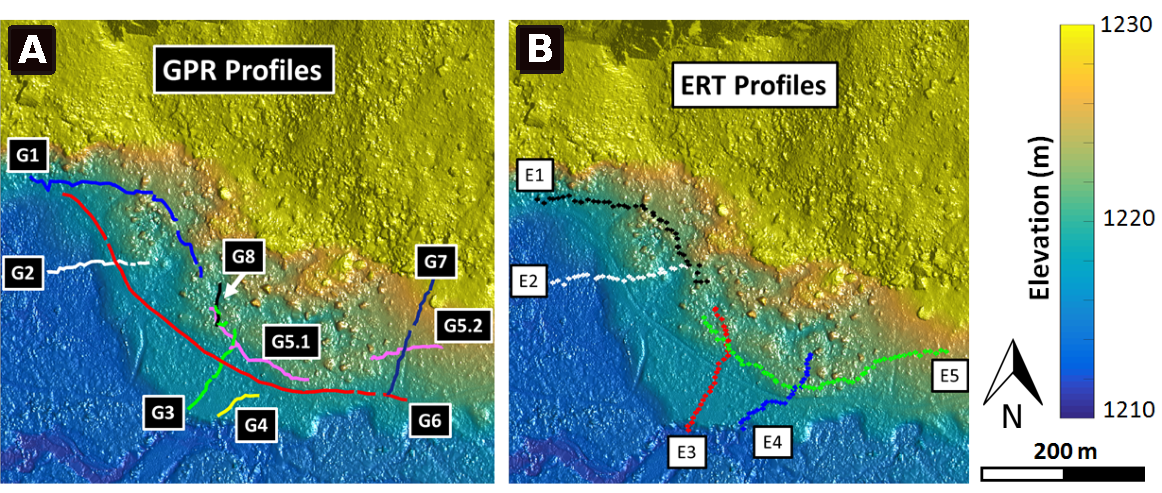
\includegraphics[width=\textwidth]{Figures/GPR_ERT_Map.pdf}
		\caption{of two section (G5.1 and G5.2). (B) Colored dots illustrate ERT transects at the study area (each individual dot represents an electrode position). Coordinate 0:0 is centered at zone 11S: Easting 274170 m and Northing 4180400 m.  \label{GPR profile 7}}

											\end{figure*}										
											
												
												
		\subsection{Electro Resistivity Tomography (ERT)}

Electrical Resistivity Tomography operates by sensing the apparent resistivity of the subsurface. In the field, we insert electrodes (metal stakes) into the surface, then we plug them in a cable, and plug the cable in a battery. Lastly, we run electrical current trough the electrodes and measure the potential difference. This then give us values of apparent resistivity. Finally, to convert the values from apparent resistivity to real resistivity, we run an inversion.

Five ERT transects were collected at the study area (Figure 27) using the Advanced Geosciences Inc SuperSting R1 (28 electrodes). An electrode spacing of six meters was adopted. Profiles E2, E3 and E4 were collected with the simple profile scheme (fixed position for all 28 electrodes) and for profiles E1 and E5 we used the roll-along profile scheme (Table 1). When using roll-along, we first collect data with all the electrodes in a fixed position, then we move the first 14 electrodes of the profile to the end of the profile and resume data collection, this step can be repeated multiple times.
the ERT data were inverted using BERT / GIMLi (Guenther \& Ruecker, (2017) and R\"ucker, G\"unther, \& Wagner, (2017).

	
	\subsection{Constraining ERT with GPR}
										
GPR profiles G1, G2, G3, G4, G5 were collected following the same path of ERT profiles E1, E2, E3, E4, and E5. this allowed us to verify the reliability of the data collected, not only by comparing the respective profiles but also by combining them. Qualitatively, we compared each GPR profile with its respective ERT profile, and quantitatively, we used the GPR profiles as regularization to improve the ERT inversion, detailed information about this technique can be found at Doetsch et al., (2012).

\COMON do we wanna a paragraph here illustrating an example how we did it with a figure?\COMOFF
									
									
									
									
									
\section{Results}
										
Our results were obtained from the analysis of eight GPR and five ERT processed profiles. And from this data we were able to identify the interface between the bottom of the Royal Arches Meadow Rock Avalanche and the palleo-valley floor. We were also able to infer the extent of the avalanche deposit.  

In order to identify the interface between the bottom of the rock avalanche depposit and paleo-valley floor using GPR and ERT, we had to look for:

\begin{itemize}
    \item In the GPR profiles: a continuous reflector in multiple directions in the hundreds of meters scale.
    \item In the ERT profiles: a sharp contrast between high resistivity material (rock avalanche deposit) overlaying conductive material (paleo-valley floor sediments).
\end{itemize}



		\subsection {GPR Results}
										
Since the rock avalanche studied here has a large surficial expression (hundreds of meters scale), we expect that its expression in the subsurface would be similar or even larger. Following this line of reasoning, we browsed the GPR profiles for continuous reflectors along and across profiles that could possibly represent the bottom of the rock avalanche. 

We started the identification process at profiles G3,  G4, and G6 where the expression of four reflectors can be easily tracked along the profiles. The elevation of such reflectors are respectively similar among other profiles and we named them Kappa, Alpha, Beta and Gamma. (Figure~\ref{Profiles_G3_G4_G6}). 

								 \begin{figure*}[h]

	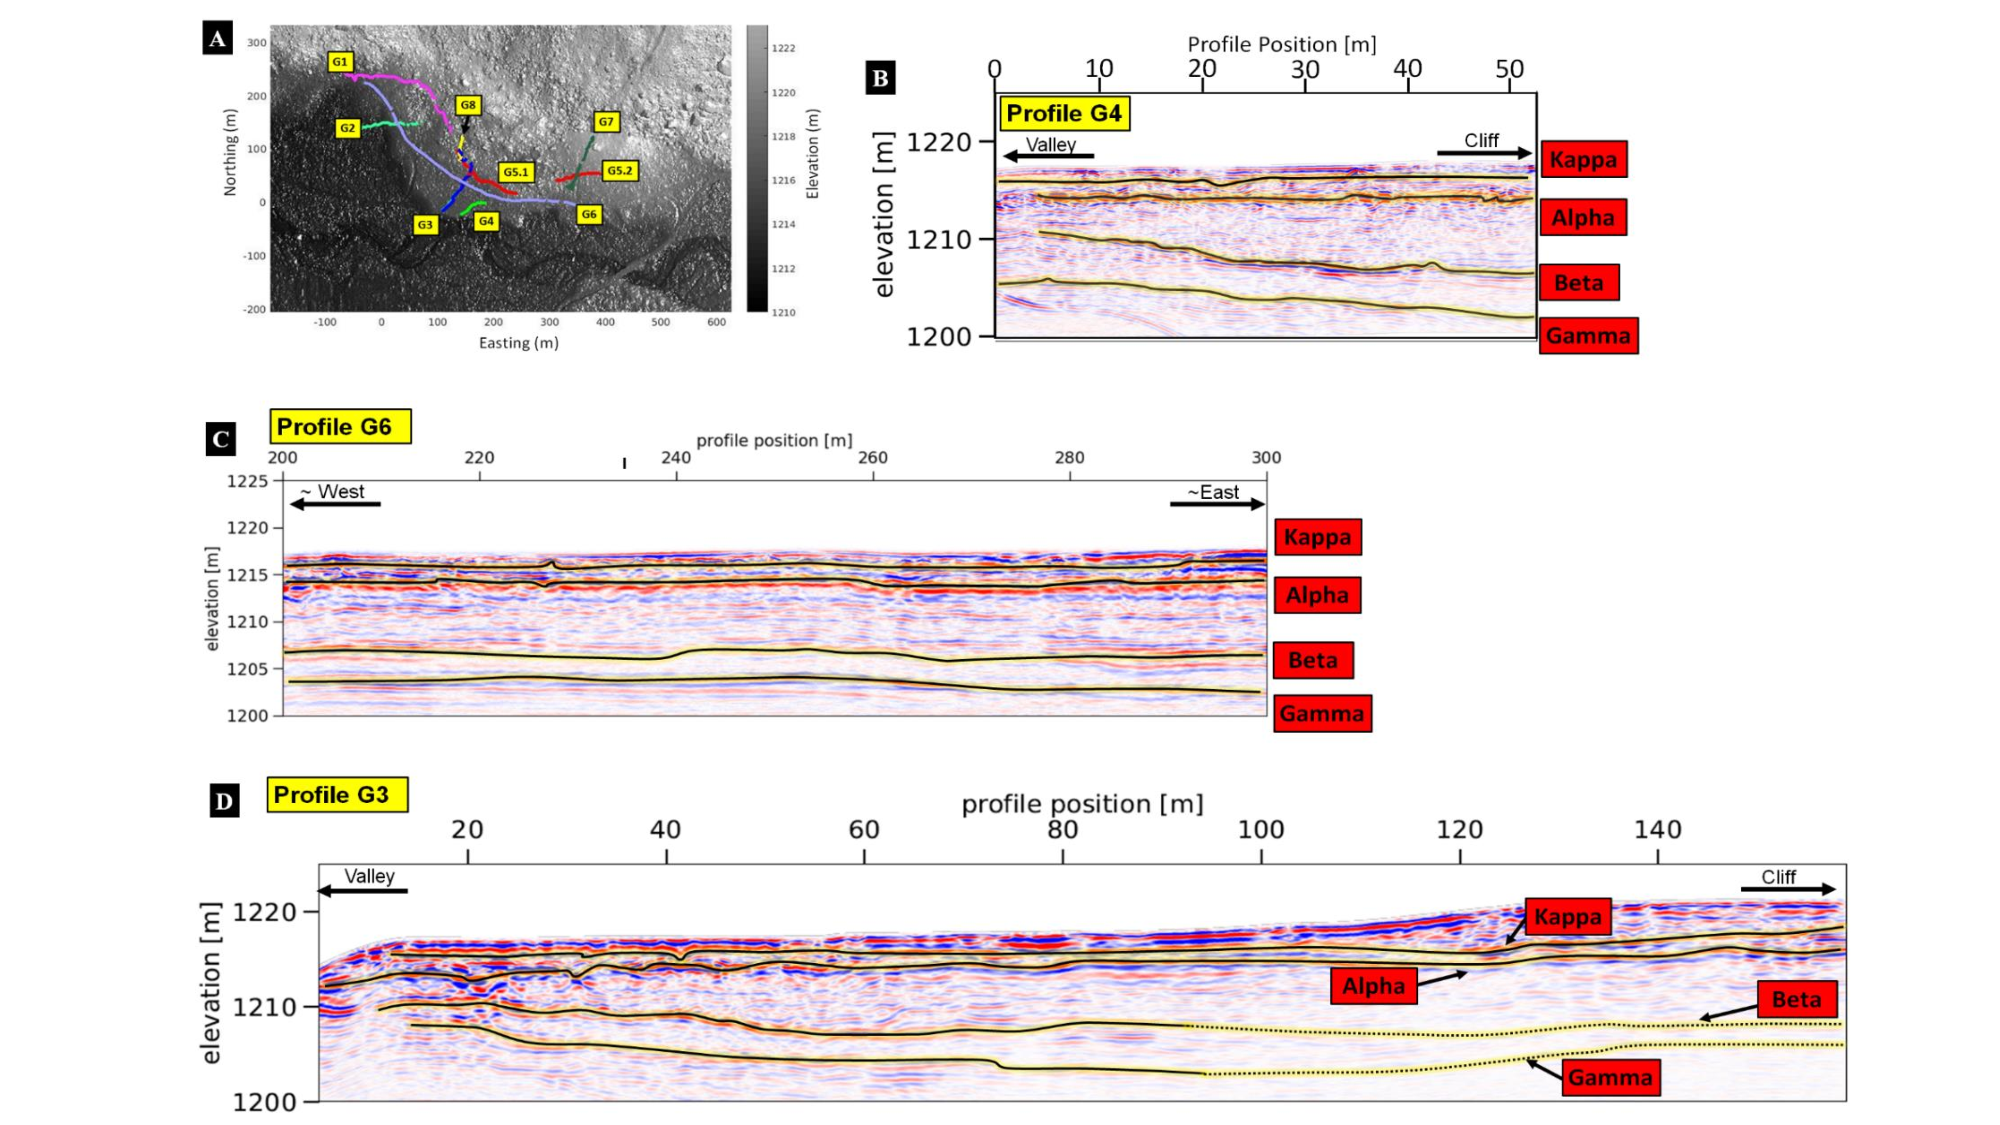
\includegraphics[width=\textwidth]{Figures/Profiles_G3_G4_G6.pdf}
		\caption{: (A) map view showing the position of the GPR profiles, (B) profile G4, (C) section of profile G6 and (D) profile G3. Yellow lines highlight the position along the profile of reflectors Alpha, Beta and Gamma. \label{Profiles_G3_G4_G6}}

								   \end{figure*}
								   
The similar elevation presented by those four reflectors is an indicative that they are continuous not only along their profile but also across profiles. And to verify the lateral continuity of those reflectors and their respective elevation, we plotted all the profiles in perspective and tracked the same four reflectors along and across profiles (Figure~\ref{Profiles_G3_G6}).						   
								   
								   \begin{figure*}[h]

	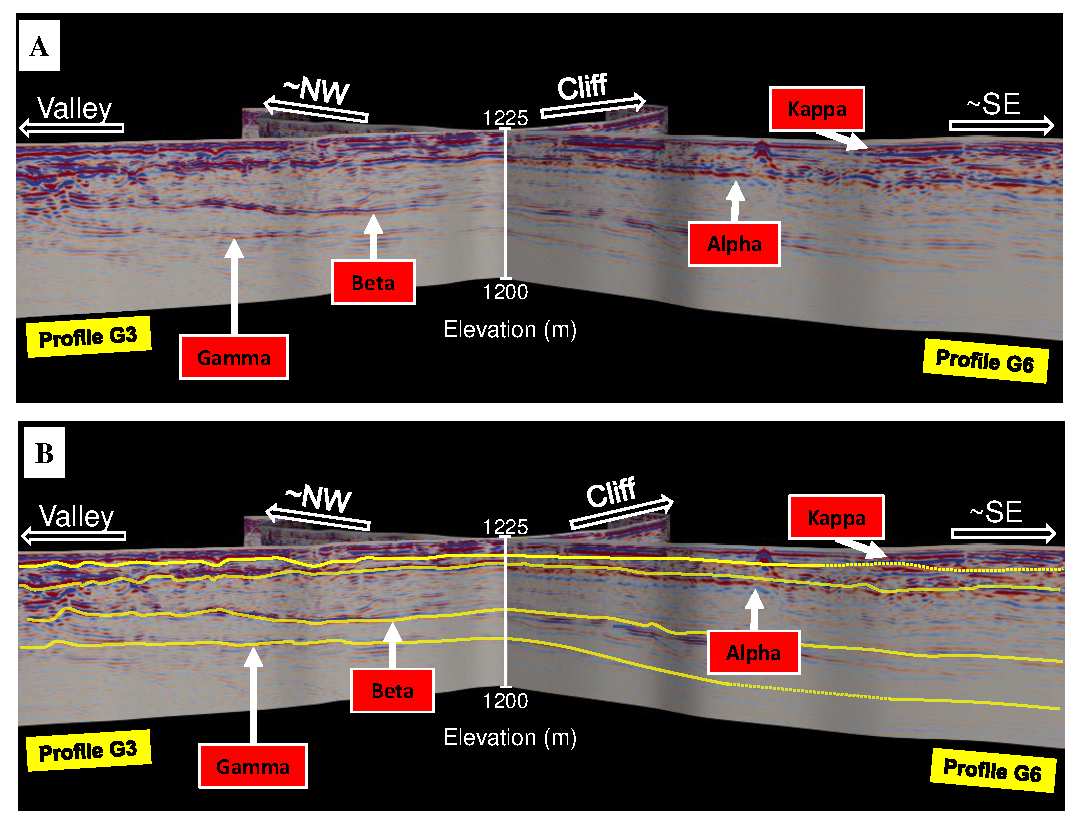
\includegraphics[width=\textwidth]{Figures/Profiles_G3_G6.pdf}
		\caption{: Three-dimensional view of profile G3 crossing profile G6. (A) continuous reflectors identified across GPR profiles. (B) Lateral continuity of reflectors Kappa, Alpha, Beta, and Gamma highlighted with yellow lines. Inferred continuity of the reflectors marked as dotted yellow line.  \label{Profiles_G3_G6}}

								   \end{figure*}
	
This approach confirmed the lateral continuity of those reflectors, and  a quantitatively analysis reveled their elevation information\COMON Table 1 \COMOFF
	

    \subsection {ERT Results}

The four reflectors identified in the GPR profiles satisfy the premise of a "continuous reflector in multiple directions in the hundreds of meters scale" as bottom of the rock avalanche deposit. Therefore, to distinguish wihch of those reflectors is indeed the bottom of the rock avalanche we looked into the ERT inversion results contrained with GPR reflectors \COMON Figure ERT + Reflectors \COMOFF. It is expected that the boundary between the rock avalanche material and the paleo-valley floor would present a sharp contrast between resistive and conductive material (respectively). And reflector Beta, at elevation \COMON 1207.06m more or less 1.1  \COMOFF marks such transition. 

										
\section{Interpretation}

    \subsection{Radarfaceis}


    \subsection{Post Glacial Rate of Deposition?}
    
		
										
				
				
										
\section{Discussion?}
										
										
										
										
										
\section{Conclusions}




\bibliography{mybibfile}

\end{document}
